\input{../mac/head-default.tex}
\input{../mac/maths.tex}

\usepackage{tikz}
\usetikzlibrary{automata,decorations.markings}
\newcommand*{\pt}{5mm}
\newcommand*{\lemautorefname}{Lemma}
\newcommand*{\thmautorefname}{Theorem}

\Bdc{Notes on the Theory of Computation}

\section{Automata and Formal Languages}

An {\bf alphabet} is a finite set \(\Sigma\), and a {\bf word over the alphabet
\(\Sigma\)} is a finite sequence of the elements of \(\Sigma\). If a word \(w\)
is the sequence \((w_0, \ldots, w_n)\) for some \(n \in \setnat\), we may write
the word as the concatenation \(w_0 \cdots w_n\). The empty word is denoted by
\(\epsilon\). The set of all words over \(\Sigma\) is
\(\Sigma^*\)\footnote{\(^*\) denotes the unary operator of Kleene star, defined
as \(A^* = \set{a_0 \cdots a_n : n \in \setnat \land \forall \, i \in \Nln[n +
1] \, (a_i \in A)} \cup \set{\epsilon}\).}. A {\bf formal language over the
alphabet \(\Sigma\)} is a subset of \(\Sigma^*\).

An {\bf automaton} is an ordered sequence that {\bf accepts} some words over an
alphabet. The set of words an automaton accepts forms a language, which is
unique, in which case we say the automaton {\bf recognises} the language. Given
an automaton \(M\), we may speak of the unique language recognised by \(M\) as
the {\bf language of the automaton \(M\)}. An automaton may accept no word, in
which case the language thereof is \(\nset\).

\subsection{Finite-State Automata and Regular Languages}

\subsubsection{Deterministic Finite-State Automata}

\Bdf
    A {\bf deterministic finite-state automaton} is an ordered quintuple
    \((\Sigma, S, \delta, s_0, F)\) wherein
    \begin{enumerate}
        \item \(\Sigma\) is an alphabet,
        \item \(S\) is a finite set of {\bf states},
        \item \(\map{\delta}{S \times \Sigma}{S}\) is the {\bf transition
        function},
        \item \(s_0 \in S\) is the {\bf initial state}, and
        \item \(F \subseteq S\) is the set of {\bf accepting states}.
    \end{enumerate}
\Edf

Let \(M = (\Sigma, S, \delta, s_0, F)\) be a deterministic finite-state
automaton and let \(w = w_0 \cdots w_n\) wherein \(n \in \setnat\) be a word
over \(\Sigma\).  Then \(M\) accepts \(w\) if there exists a sequence of states
\((r_0, \ldots, r_{n + 1})\) in \(S\) such that
\begin{enumerate}
    \item \(r_0 = s_0\),
    \item \(\delta(r_i, w_i) = r_{i + 1}\) for \(i \in \Nln[n + 1]\), and
    \item \(r_{n + 1} \in F\).
\end{enumerate}
Furthermore, \(M\) accepts \(\epsilon\) if \(s_0 \in F\).

\subsubsection{Nondeterministic Finite-State Automata}

\Bdf
    A {\bf nondeterministic finite-state automaton} is an ordered quintuple
    \((\Sigma, S, \delta, s_0, F)\) wherein
    \begin{enumerate}
        \item \(\Sigma\) is an alphabet,
        \item \(S\) is a finite set of states,
        \item \(\map{\delta}{S \times (\Sigma \cup \set{\epsilon})}{\pow(S)}\)
        is the transition function,
        \item \(s_0 \in S\) is the initial state, and
        \item \(F \subseteq S\) is the set of accepting states.
    \end{enumerate}
\Edf

Let \(M = (\Sigma, S, \delta, s_0, F)\) be a nondeterministic finite-state
automaton and let \(w\) be a word over \(\Sigma\). Then \(M\) accepts \(w\) if
\(w = w_0 \cdots w_n\) wherein \(n \in \setnat\) such that each \(w_i \in \Sigma
\cup \set{\epsilon}\) for \(i \in \Nln[n + 1]\) and that there exists a sequence
of states \((r_0, \ldots, r_{n + 1})\) in \(S\) such that
\begin{enumerate}
    \item \(r_0 = s_0\),
    \item \(r_{i + 1} \in \delta(r_i, w_i)\) for \(i \in \Nln[n + 1]\), and
    \item \(r_{n + 1} \in F\).
\end{enumerate}

We say that two automata are equivalent if they recognise the same language.

\Bth
    \label{thm1}
    Every nondeterministic finite-state automaton has an equivalent
    deterministic finite-state automaton.
\Eth
\Bpr
    Let \(N = (\Sigma, S, \delta, s_0, F)\) be the nondeterministic finite-state
    automaton recognising some language \(A\) over \(\Sigma\).  We construct a
    deterministic finite-state automaton \(M = (\Sigma, S', \delta', s_0', F')\)
    recognising \(A\).

    We first see that \(S' = \pow(S)\) and that \(F' = \set{R \in S' : R \cap F
    \neq \nset}\).

    Let \(\map{\delta_0}{S \times \set{\epsilon}}{\pow(S)}\) be defined as
    \(\delta_0(s, \epsilon) = \delta(s, \epsilon)\) for each \(s \in S\). Assume
    first that, thus induced, \(\delta_0 = \nset\) for \(N\). For each \(R \in
    S'\) and for each \(a \in \Sigma\), let \(\delta'(R, a) = \set*{s \in S :
    \exists \, r \in R \, \big(s \in \delta(r, a)\big)}\). Equivalently,
    \[
        \delta'(R, a) = \bigcup_{r \in R} \delta(r, a).
    \]
    Also let \(s_0' = \set{s_0'}\). We then see that \(M = (\Sigma, S', \delta',
    s_0', F')\) recognises \(A\).

    Assume then that \(\delta_0 \neq \nset\) for \(N\). For each \(Q \subseteq S
    \), let
    \[
        E(Q) = \set*{s \in S : \exists \, n \in \setnat \, \exists \, r \in Q \,
        \big(s = \delta^n(r, \epsilon)\big)}.
    \]
    We then let
    \[
        \delta'(Q, a) = \set*{s \in S : \exists \, r \in Q \, s \in
        E\big(\delta(r, a)\big)}
    \]
    and let \(s_0' = E(\set{s_0})\). We similarly see that \(M = (\Sigma, S',
    \delta', s_0', F')\) recognises \(A\).

    Therefore, the theorem holds.
\Epr

\subsubsection{Regular Expressions and Regular Languages}

\Bdf
    Let \(\Sigma\) be an alphabet, and let \(a \in \Sigma\). Then \(R\) is a
    {\bf regular expression over \(\Sigma\)} if
    \begin{enumerate}
        \item \(R = \nset\),
        \item \(R = \epsilon\),
        \item \(R = a\),
        \item \(R = R_1 \cup R_2\) wherein \(R_1\) and \(R_2\) are regular
        expressions over \(\Sigma\),
        \item \(R = R_1 R_2\)\footnote{\(R_1 R_2\) denotes the concatenation of
        \(R_1\) and \(R_2\).} wherein \(R_1\) and \(R_2\) are regular
        expressions over \(\Sigma\), or
        \item \(R = R_1^*\) wherein \(R_1\) is a regular expression over
        \(\Sigma\).
    \end{enumerate}
\Edf

The language described by a regular expression is a {\bf regular language}. Each
regular expression describes a unique regular language, while a regular language
may have multiple distinct regular expressions describing it. If \(R\) is a
regular expression, we denote the regular language it describes by \(L(R)\).

Let \(\Sigma\) be an alphabet, let \(a \in \Sigma\), and let \(R\), \(R_1\), and
\(R_2\) be regular expressions over \(\Sigma\). If \(R = \nset\), then \(L(R) =
\nset\). If \(R = \epsilon\), then \(L(R) = \set{\epsilon}\). If \(R = a\), then
\(L(R) = \set{a}\). If \(R = R_1 \cup R_2\), then \(L(R) = L(R_1) \cup L(R_2)\).
If \(R = R_1 R_2\), then \(L(R) = L(R_1) L(R_2)\)\footnote{If \(A\) and \(B\)
are languages, \(A B\) denotes the concatenation of \(A\) and \(B\), defined
as \(A B = \set{a b : a \in A \land b \in B}\).}. If \(R = R_1^*\), then \(L(R) =
L(R_1)^*\).

\subsubsection{Equivalence Between Finite-State Automata and Regular Languages}

\Blm
    \label{lem1}
    If a language is regular, then some nondeterministic finite-state automaton
    recognises it.
\Elm
\Bpr
    Let \(\Sigma\) be an alphabet, let \(A\) be a regular language over
    \(\Sigma\), and let \(R\) be a regular expression which describes \(A\).

    If \(R = \nset\), then the nondeterministic finite-state automaton \(N\)
    characterised by the following diagram recognises \(A\).
    \begin{figure}[!h]
        \centering
        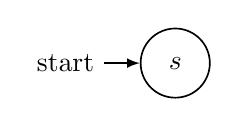
\begin{tikzpicture}[
            ->,>=latex,auto,semithick,
            node distance=2.5cm
        ]
        \node[initial,state] (s) {\(s\)};
        \end{tikzpicture}
    \end{figure}

    \noindent Equivalently, \(N = (\Sigma, \set{s}, \delta, s, \nset)\) wherein
    \(\delta(r, b) = \nset\) for any \(r\) and \(b\).

    If \(R = \epsilon\), then the nondeterministic finite-state automaton \(N\)
    characterised by the following diagram recognises \(A\).
    \begin{figure}[!h]
        \centering
        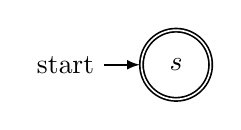
\begin{tikzpicture}[
            ->,>=latex,auto,semithick,
            node distance=2.5cm
        ]
        \node[initial,state,accepting] (s) {\(s\)};
        \end{tikzpicture}
    \end{figure}

    \noindent Equivalently, \(N = (\Sigma, \set{s}, \delta, s, \set{s})\)
    wherein \(\delta(r, b) = \nset\) for any \(r\) and \(b\).

    If \(R = a\) for some \(a \in \Sigma\), then the nondeterministic
    finite-state automaton \(N\) characterised by the following diagram
    recognises it.
    \begin{figure}[!h]
        \centering
        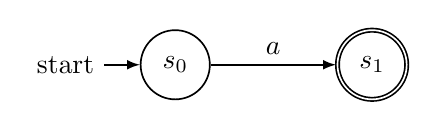
\begin{tikzpicture}[
            ->,>=latex,auto,semithick,
            node distance=2.5cm
        ]
        \node[initial,state] (s0) {\(s_0\)};
        \node[state,accepting] (s1) [right of=s0] {\(s_1\)};
        \path (s0) edge node {\(a\)} (s1);
        \end{tikzpicture}
    \end{figure}

    \noindent Equivalently, \(N = (\Sigma, \set{s_0, s_1}, \delta, s_0,
    \set{s_1})\) wherein \(\delta(s_0, a) = \set{s_1}\) and \(\delta(r, b) =
    \nset\) if \(r \neq s_0\) or \(b \neq a\).

    Assume that \(R_1\) and \(R_2\) are regular expressions over \(\Sigma\),
    that \(N_1 = (\Sigma, S_1, \delta_1, s_1, F_1)\) is a nondeterministic
    finite-state automaton recognising \(L(R_1)\), and that \(N_2 = (\Sigma,
    S_2, \delta_2, s_2, F_2)\) is a nondeterministic finite-state automaton
    recognising \(L(R_2)\).

    If \(R = R_1 \cup R_2\), let \(s_0\) be a state not in \(S_1\) or \(S_2\),
    let \(S = S_1 \cup s_2 \cup \set{s_0}\), and let \(F = F_1 \cup F_2\).
    Define \(\map{\delta}{S \times (\Sigma \cup \set{\epsilon})}{\pow(S)}\) so
    that for each \(r \in S\) and each \(b \in \Sigma \cup \set{\epsilon}\) we
    have
    \[
        \delta(r, b) = \begin{cases}
            \delta_1(r, b) & \text{if }\ r \in S_1,\\
            \delta_2(r, b) & \text{if }\ r \in S_2,\\
            \set{s_1, s_2} & \text{if }\ r = s_0 \land b = \epsilon \text{,
            and}\\
            \nset & \text{otherwise.}
        \end{cases}
    \]
    We see that \(N = (\Sigma, S, \delta, s_0, F)\) is a nondeterministic
    finite-state automaton recognising \(A\).

    If \(R = R_1 R_2\), let \(S = S_1 \cup S_2\). Define \(\map{\delta}{S \times
    (\Sigma \cup \set{\epsilon})}{\pow(S)}\) so that for each \(r \in S\) and
    each \(b \in \Sigma \cup \set{\epsilon}\) we have
    \[
        \delta(r, b) = \begin{cases}
            \delta_1(r, b) & \text{if }\ (r \in S_1 \land r \not\in F_1) \lor (r
            \in F_1 \land b \neq \epsilon),\\
            \delta_1(r, b) \cup \set{s_2} & \text{if }\ r \in F_1 \land b =
            \epsilon \text{, and}\\
            \delta_2(r, b) & \text{otherwise.}
        \end{cases}
    \]
    We see that \(N = (\Sigma, S, \delta, s_1, F_2)\) is a nondeterministic
    finite-state automaton recognising \(A\).

    If \(R = R_1^*\), let \(s_0\) be a state not in \(S_1\), let \(S = S_1 \cup
    \set{s_0}\), and let \(F = F_1 \cup \set{s_0}\). Define \(\map{\delta}{S
    \times (\Sigma \cup \set{\epsilon})}{\pow(S)}\) so that for each \(r \in S\)
    and each \(b \in \Sigma \cup \set{\epsilon}\) we have
    \[
        \delta(r, b) = \begin{cases}
            \delta_1(r, b) & \text{if }\ (r \in S_1 \land r \not\in F_1) \lor (r
            \in F_1 \land b \neq \epsilon),\\
            \delta_1(r, b) \cup \set{s_1} & \text{if }\ r \in F_1 \land b =
            \epsilon,\\
            \set{s_1} & \text{if }\ r = s_0 \land b = \epsilon \text{, and}\\
            \nset & \text{otherwise.}
        \end{cases}
    \]
    We see that \(N = (\Sigma, S, \delta, s_0, F)\) is a nondeterministic
    finite-state automaton recognising \(A\).

    Therefore, the lemma holds by the principle of induction.
\Epr

\Bdf
    A {\bf generalised nondeterministic finite-state automaton} is an ordered
    quintuple \((\Sigma, S, \delta, s_0, s_1)\) wherein
    \begin{enumerate}
        \item \(\Sigma\) is an alphabet,
        \item \(S\) is a finite set of states,
        \item \(\map{\delta}{(S \setminus \set{s_1}) \times (S \setminus
        \set{s_0})}{\mathcal{R}}\) wherein \(\mathcal{R}\) is the set of all
        regular expressions over \(\Sigma\) is the transition function,
        \item \(s_0 \in S\) is the initial state, and
        \item \(s_1 \neq s_0 \in S\) is the accepting state.
    \end{enumerate}
\Edf

Let \(M = (\Sigma, S, \delta, s_0, s_1)\) be a generalised nondeterministic
finite-state automaton and let \(w\) be a word over \(\Sigma\). Then \(M\)
accepts \(w\) if \(w = w_0 \cdots w_n\) wherein \(n \in \setnat\) such that each
\(w_i \in \Sigma^*\) for \(i \in \Nln[n + 1]\) and that there exists a sequence
of states \((r_0, \ldots, r_{n + 1})\) in \(S\) such that
\begin{enumerate}
    \item \(r_0 = s_0\),
    \item \(r_{n + 1} = s_1\), and
    \item \(w_i \in L(R_i)\) wherein \(R_i = \delta(r_i, r_{i + 1})\) for \(i
    \in \Nln[n + 1]\).
\end{enumerate}

\Blm
    \label{lem2}
    If a nondeterministic finite-state automaton recognises a language, then it
    is regular.
\Elm
\Bpr
    Let \(N = (\Sigma, S, \delta, s_0, F)\) be a nondeterministic finite-state
    automaton recognising the language \(A\) over \(\Sigma\). We argue that
    \(A\) is described by some regular expression \(R\) over \(\Sigma\).

    Let \(G = (\Sigma, S', \delta', s_0', s_1')\) be a generalised
    nondeterministic finite-state automaton such that
    \begin{enumerate}
        \item \(s_0' \not\in S\),
        \item \(s_1' \not\in S\),
        \item \(S' = S \cup \set{s_0', s_1'}\), and
        \item for each \(r_0 \in S \cup \set{s_0'}\) and each \(r_1 \in S \cup
        \set{s_1'}\) we have
            \[
                \delta'(r_0, r_1) = \begin{cases}
                        \epsilon & \text{if }\ (r_0 = s_0' \land r_1 = s_0) \lor
                        (r_0 \in F \land r_1 = s_1'),\\
                        R' & \text{if }\ r_0 \in S \land r_1 \in S \land \forall
                        \, r \in L(R') \, \big(r_1 \in \delta(r_0, r)\big)
                        \text{, and}\\
                        \nset & \text{otherwise.}
                    \end{cases}
            \]
    \end{enumerate}
    We see that \(G\) also recognises \(A\). We shall then convert \(G\) into
    regular expression \(R\).

    Let \(k = \abs{S'}\).

    If \(k = 2\), then \(S' = \set{s_0', s_1'}\), and so \(R = \delta'(s_0',
    s_1')\) is the regular expression.

    If \(k > 2\), let \(s \in S'\) be distinct from \(s_0'\) and \(s_1'\), and
    let \(G' = (\Sigma, S'', \delta'', s_0', s_1')\) be a generalised
    nondeterministic finite-state automaton such that
    \begin{enumerate}
        \item \(S'' = S' \setminus \set{s}\),
        \item for each \(r_0 \in S'' \setminus \set{s_0'}\) and each \(r_1 \in
        S'' \setminus \set{s_1'}\) we have
        \[
            \delta''(r_0, r_1) = R_0 R_1^* R_2 \cup R_3
        \]
        wherein \(R_0 = \delta'(r_0, s)\), \(R_1 = \delta'(s, s)\), \(R_2 =
        \delta'(s, r_1)\), and \(R_3 = \delta'(r_0, r_1)\).
    \end{enumerate}
    We see that \(G'\) is equivalent to \(G\).

    Because \(G'\) has one fewer state than \(G\), by the principle of
    induction, there exists regular expression \(R\) converted from \(G\) for
    any generalised nondeterministic finite-state automaton.

    Therefore, the lemma holds.
\Epr

\Bth
    \label{thm2}
    A language is regular if and only if some nondeterministic finite-state
    automaton recognises it.
\Eth
\Bpr
    The theorem holds by \autoref{lem1} and \autoref{lem2}.
\Epr

\Bcr
    A language is regular if and only if some deterministic finite-state
    automaton recognises it.
\Ecr
\Bpr
    The corollary holds by \autoref{thm1} and \autoref{thm2}.
\Epr

\subsubsection{Nonregular Languages}

\Bth[pumping lemma]
    If \(A\) is a regular language over \(\Sigma\), then there is a \(p \in
    \posint\), the \textbf{\textit{pumping length}}, such that if \(w \in A\) is
    of length at least \(p\), then there exist \(x\), \(y\), and \(z \in
    \Sigma^*\) which satisfy
    \begin{enumerate}
        \item \(w = x y z\),
        \item \(x y^i z \in A\) for each \(i \in \setnat\),
        \item \(\abs{y} > 0\), and
        \item \(\abs{x y } \leq p\).
    \end{enumerate}
\Eth
\Bpr
    Let \(M = (\Sigma, S, \delta, s_0, F)\) be a deterministic finite-state
    automaton recognising \(A\) and let \(p = \abs{S}\).

    Let \(w = w_0 \cdots w_n\) wherein \(n \in \setnat\) be a word in \(R\) of
    length \(n + 1\) which satisfies \(n + 1 \geq p\). Let \(r_0, \ldots, r_{n +
    1}\) be the sequence of states that \(M\) enters when accepting \(r\). This
    sequence has length \(n + 2\), which must be at least \(p + 1\). Among the
    first \(p + 1\) elements in the sequence, two must be the same state by the
    pigeonhole principle. Let the first of these be \(r_i\) and the second
    \(r_j\). We note that \(i \leq j - 1\) and that \(j \leq p\). Now let \(x =
    w_0 \cdots w_{i - 1}\), \(y = w_i \cdots w_{j - 1}\), and \(z = w_j \cdots
    w_n\).

    Thus induced, \(r = x y z\) satisfies the pumping lemma.
\Epr

We may use the pumping lemma to prove that a language is not regular. To do so,
first assume that the language is regular, and then use the pumping lemma to
guarantee the existence of a pumping length \(p\) such that all words of length
\(p\) or greater in the language can be pumped. Next, find a word in the
language with length \(p\) or greater but cannot be pumped. Finally, demonstrate
that this word cannot be pumped by considering all ways of diving it into three
such substrings described by the pumping lemma. The existence of this word
contradicts the pumping lemme assuming the language is regular. Hence, the
language is not regular.

\subsection{Pushdown Automata and Context-Free Languages}

\subsubsection{Pushdown Automata}

\Bdf
    A {\bf pushdown automaton} is an ordered sextuple \((\Sigma, \Gamma, S,
    \delta, s_0, F)\) wherein
    \begin{enumerate}
        \item \(\Sigma\) is an alphabet, for the input,
        \item \(\Gamma\) is another alphabet, for the {\bf stack},
        \item \(S\) is a finite set of states,
        \item \(\map{\delta}{S \times (\Sigma \cup \set{\epsilon}) \times
        (\Gamma \cup \set{\epsilon})}{\pow\big(S \times (\Gamma \cup
        \set{\epsilon})\big)}\) is the transition function,
        \item \(s_0 \in S\) is the initial state, and
        \item \(F \subseteq S\) is the set of final or accepting states.
    \end{enumerate}
\Edf

Let \(M = (\Sigma, \Gamma, S, \delta, s_0, F)\) be a pushdown automaton and let
\(w\) be a word over \(\Sigma\). Then \(M\) accepts \(w = w_0 \cdots w_n\)
wherein \(n \in \setnat\) such that \(w_i \in \Sigma \cup \set{\epsilon}\) for
\(i \in \Nln[n + 1]\) and that there exist a sequence of states \((r_0, \ldots,
r_{n + 1})\) in \(S\) and a sequence of words \((q_0, \ldots, q_{n + 1})\) in
\(\Gamma^*\) such that
\begin{enumerate}
    \item \(r_0 = s_0\),
    \item \(q_0 = \epsilon\),
    \item \((r_{i + 1}, b) \in \delta(r_i, w_i, a)\), \(q_i = a t\), and \(q_{i
    + 1} = b t\) for some \(a\) and \(b \in \Gamma \cup \set{\epsilon}\) and
    some \(t \in \Gamma^*\) for \(i \in \Nln[n + 1]\), and
    \item \(r_{n + 1} \in F\).
\end{enumerate}

\Bxr
    Let \(\Sigma = \set{0, 1}\) be an alphabet. Construct a pushdown automaton
    which recognises the language \(\set{0^n 1^n : n \in \setnat}\).
\Exr
\Bsl
    The pushdown automaton \(M\) characterised by the following diagram
    recognises the given language.
    \begin{figure}[!h]
        \centering
        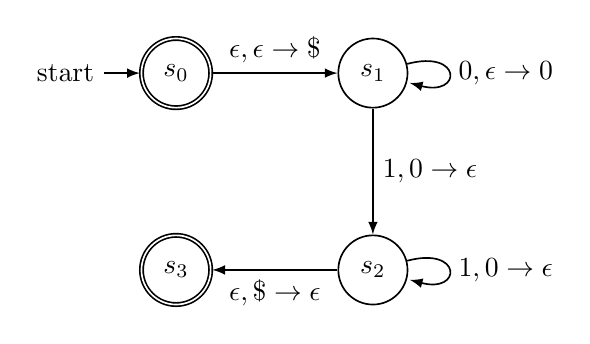
\begin{tikzpicture}[
            ->,>=latex,auto,semithick,
            node distance=2.5cm
        ]
        \node[initial,state,accepting] (s0) {\(s_0\)};
        \node[state] (s1) [right of=s0] {\(s_1\)};
        \node[state] (s2) [below of=s1] {\(s_2\)};
        \node[state,accepting] (s3) [left of=s2] {\(s_3\)};
        \path (s0) edge node {\(\epsilon, \epsilon \to \$\)} (s1)
        (s1) edge node {\(1, 0 \to \epsilon\)} (s2)
        edge [loop right] node {\(0, \epsilon \to 0\)} ()
        (s2) edge node {\(\epsilon, \$ \to \epsilon\)} (s3)
        edge [loop right] node {\(1, 0 \to \epsilon\)} ();
        \end{tikzpicture}
    \end{figure}

    \noindent Equivalently, \(M = (\Sigma, \Gamma, S, \delta, s_0, F)\)
    wherein
    \begin{enumerate}
        \item \(\Gamma = \set{0, \$}\),
        \item \(S = \set{s_0, s_1, s_2, s_3}\),
        \item \(F = \set{s_0, s_3}\), and
        \item for each \(s \in S\), each \(a \in \Sigma \cup
            \set{\epsilon}\), and each \(b \in \Gamma \cup
            \set{\epsilon}\) we have
            \[
                \delta(s, a, b) = \begin{cases}
                    \set{(s_1, \$)} & \text{if } s = s_0 \land a = \epsilon
                    \land b = \epsilon,\\
                    \set{(s_1, 0)} & \text{if } s = s_1 \land a = 0 \land b =
                    \epsilon,\\
                    \set{(s_2, \epsilon)} & \text{if } (s = s_1 \lor s = s_2)
                    \land a = 1 \land b = 0,\\
                    \set{(s_3, \epsilon)} & \text{if } s = s_2 \land a =
                    \epsilon \land b = \$ \text{, and}\\
                    \nset & \text{otherwise}
                \end{cases}
            \]
    \end{enumerate}
    is a pushdown automaton which recognises the given language.
\Esl

\subsubsection{Context-Free Grammars and Context-Free Languagse}

\Bdf
    A {\bf context-free grammar} is an ordered quadruple \((\Sigma, V, R, S)\)
    wherein
    \begin{enumerate}
        \item \(\Sigma\) is an alphabet, the elements whereof are {\bf
        terminals},
        \item \(V\) is another alphabet, the elements whereof are {\bf
        variables}, which is disjoint from \(\Sigma\),
        \item \(\map{R}{V}{(\Sigma \cup V)^*}\) is a finite set of {\bf
        production rules}, and
        \item \(S \in V\) is the {\bf start variable}.
    \end{enumerate}
\Edf

Let \((\Sigma, V, R, S)\) be a context-free grammar. If \((A, w)\) wherein \(A
\in V\) and \(w \in (\Sigma \cup V)^*\) is a production rule, we write \(A \to
w\). If \(u\), \(v\), and \(w \in (\Sigma \cup V)^*\), and \(A \to w\) is a
production rule of the grammar, we say that \(u A v\) {\bf yields} \(u w v\),
written \(u A v \Rightarrow u w v\). We say that \(u\) {\bf derives} \(v\),
written \(u \Rightarrow^* v\), if \(u = v\), \(u \Rightarrow v\), or there
exists a sequence \((u_0, \ldots, u_n)\) wherein \(n \in \setnat\) such that
\[
    u \Rightarrow u_0 \Rightarrow \cdots \Rightarrow u_n \Rightarrow v.
\]
If \(A \to u\) and \(A \to v\) are production rules of the grammar, we may
denote them by \(A \to u \, | \, v\). The {\bf language of the grammar} is
\(\set{w \in \Sigma^* : S \Rightarrow^* w}\).

The language of a context-free grammar is a {\bf context-free language}.

\Bxr
    Let \(\Sigma = \set{0, 1}\) be an alphabet. Construct a context-free grammar
    whose language is \(\set{0^n 1^n : n \in \setnat}\).
\Exr
\Bsl
    Let \((\Sigma, V, R, S)\) be the context-free grammar wherein \(V =
    \set{S}\) and \(R\) consists of the following production rule
    \[
        S \to 0 S 1 \, | \, \epsilon.
    \]
    The language of the above context-free grammar is the given language.
\Esl

A derivation of a word in a context-free grammar is a {\bf leftmost derivation}
if at every step of production the leftmost remaining variable is the one
substituted according to a production rule.

\Bdf
    A word is derived {\bf ambiguously} in a context-free grammar if there exist
    two or more distinct leftmost derivations for it.

    A context-free grammar is {\bf ambiguous} is it generates some words
    ambiguously.
\Edf

Some context-free languages can only be generated by ambiguous context-free
grammars. Such languages are {\bf inherently ambiguous}.

\subsubsection{Chomsky Normal Form}

\Bdf
    A context-free grammar is {\bf in Chomsky normal form} if every production
    rule thereof is
    \begin{enumerate}
        \item \(S \to \epsilon\) wherein \(S\) is the start variable,
        \item \(A \to B C\) wherein \(A\), \(B\), and \(C\) are variables and
        \(B\) and \(C\) are not the start variable, or
        \item \(A \to a\) wherein \(A\) is a variable and \(a\) is a terminal.
    \end{enumerate}
\Edf

\Bth
    Any context-free language is generated by a context-free grammar in Chomsky
    normal form.
\Eth
\Bpr
    Let \((\Sigma, V, R, S)\) be a context-free grammar. We demonstrate a
    procedure to convert it into another context-free grammar in Chomsky normal
    form \((\Sigma, V', R', S')\).

    We first add \(S' \to S\) as a production rule.

    Second, if there exist rules of the form \(A \to \epsilon\) wherein \(A \neq
    S'\), we remove them and repeatedly replace any rule of the form \(B \to u A
    v\) wherein \(B \in V'\) and \(u\) and \(v \in (\Sigma \cup V')^*\) with \(B
    \to u v\) for each occurrence of \(A\).

    Third, if there exist rules of the form \(A \to B\) wherein \(A\) and \(B
    \in V'\), we remove them and replace any rule of the form \(B \to u\)
    wherein \(u \in (\Sigma \cup V')^*\) with \(A \to u\).

    Lastly, we replace each rule of the form \(A \to u_0 \cdots u_n\) wherein
    \(n \in \setnat\) and \(u_i \in \Sigma \cup V'\) for \(i \in \Nln[n + 1]\)
    such that \(n > 1\) with the rules \(A \to u_0 A_0\), \(A_0 \to u_1 A_1\),
    \ldots, \(A_{n - 2} \to u_{n - 1} u_n\) and add \(A_i\) for \(i \in \Nln[n -
    1]\) as variables. We then replace any terminal \(u_i\) for \(i \in \Nln[n +
    1]\) with the new variable \(U_i\) while adding the rule \(U_i \to u_i\).

    The resultant context-free grammar is in Chomsky normal form, and therefore
    the theorem holds.
\Epr

\subsubsection{Equivalence Between Pushdown Automata and Context-Free Languages}

\Blm
    \label{lem3}
    If a language is context-free, then some pushdown automaton recognises it.
\Elm
\Bpr
    TODO
\Epr

\Blm
    \label{lem4}
    If a pushdown automaton recognises a language, then it is context-free.
\Elm
\Bpr
    TODO
\Epr

\Bth
    A language is context-free if and only if some pushdown automaton recognises
    it.
\Eth
\Bpr
    The theorem holds by \autoref{lem3} and \autoref{lem4}.
\Epr

\Bcr
    Every regular language is context-free.
\Ecr
\Bpr
    Let \(A\) be a regular language. Let \((\Sigma, S, \delta, s_0, F)\) be a
    nondeterministic finite-state automaton recognising \(A\). Then the pushdown
    automaton \((\Sigma, \nset, S, \delta', s_0, F)\) wherein \(\delta'(s, a,
    \epsilon) = \delta(s, a)\) for each \(s \in S\) and each \(a \in \Sigma \cup
    \set{\epsilon}\) also recognises \(A\). Thus, \(A\) is context-free.
\Epr

\subsubsection{Non-Context-Free Languages}

\Bth[pumping lemma for context-free languages]
    If \(A\) is a context-free language over \(\Sigma\), then there is a \(p \in
    \posint\), the pumping length, such that if \(w \in A\) is of length at
    least \(p\), then there exist \(u\), \(v\), \(x\), \(y\), and \(z \in
    \Sigma^*\) which satisfy
    \begin{enumerate}
        \item \(w = u v x y z\),
        \item \(u v^i x y^i z \in A\) for each \(i \in \setnat\),
        \item \(\abs{v y} > 0\), and
        \item \(\abs{v x y} \leq p\).
    \end{enumerate}
\Eth
\Bpr
    TODO
\Epr

\subsubsection{Deterministic Pushdown Automata and Deterministic Context-Free
Languages}

\Edc
